\appendix


\section{Appendiks - Grunnleggende databladkunnskaper}\label{app:datablad}

For å bruke micro:bit, eller en hvilket som helst mikrokontroller, er det viktig å kunne mestre bruken av datablader. Mer spesifikt, så er det veldig viktig å forstå hvordan man bruker det som kalles memory mapped IO. I praksis, betyr memory mapped IO at man typecaster adressen til en modul inn i en \verb|struct|. Grunnen til at man bruker memory mapped IO, er at det gjør det mulig å skrive direkte til registrene i mikrokontrolleren ved å bare endre på \verb|struct|-ens medlemsvariabler. Se forøvrig pensumlitteratur og forelesninger for mer informasjon om memory mapped IO og hvordan en forholder seg til det i \verb|C|-programmering.

\subsection{Memory Mapped IO informasjon fra datablad}
Det første man trenger for å kunne typecaste adressen til en modul inn i en \verb|struct|, er å finne adressen til modulen. I \verb|GPIO|-tilfellet, er baseadressen enten \verb|0x50000000| eller \verb|0x50000300| (se figur \ref{fig:app-gpio-modul}).


\begin{figure}[ht]
    \centering
    \includegraphics[scale=0.615]{Main/figures/gpio_addresse.JPG}
    \caption{Startsadressene til GPIO-modulene (side 144 fra \texttt{nrf52833 Product Specification.pdf}.}
    \label{fig:app-gpio-modul}
\end{figure}

Som dere kan se, så har noen moduler flere \textit{instanser} av en modul. Et annet eksempel på dette er \verb|Timer|-modulen til nRF52-en. Der finnes det fem forskjellige kopier av samme enhet (se figur \ref{fig:app-timerl}). Dette er veldig nyttig dersom man ønsker for eksempel flere uavhengige klokker (ikke relevant for denne laben).

\begin{figure}[ht]
    \centering
    \includegraphics[scale=0.61]{Main/figures/timer_memory.JPG}
    \caption{Startadressene til \texttt{Timer}-modulen (side 446 fra \texttt{nrf52833 Product Specification.pdf}.}
    \label{fig:app-timerl}
\end{figure}

Når man først har baseadressen, oversettes dette ganske direkte inn i \verb|C| slik:

\verb|#define GPIO0 ((NRF_GPIO_REG0*)0x50000000)|

Denne kodesnutten tilsvarer å definere den første instansen av \verb|GPIO| som en peker til adresse \verb|0x5000000|, hvor pekeren er av typen \verb|NRF_GPIO_REG0|. 

Neste steg er å definere hvordan \verb|NRF_GPIO_REG0| ser ut. Strukturen til \verb|NRF_ GPIO_REG0| finner man som oftest rett under baseadressen (se figur \ref{fig:app-memory-struct}).

\begin{figure}[ht]
    \centering
    \includegraphics[scale=0.61]{Main/figures/memory_stuff_gpio.JPG}
    \caption{Registrene i GPIO-modulene (side 144 fra \texttt{nrf52833 Product Specification.pdf}.}
    \label{fig:app-memory-struct}
\end{figure}

Informasjonen som vi trenger for å kunne bruke \verb|NRF_GPIO_REG0| sine registre finner man under \verb|Register| og \verb|Offset|. \verb|Register| beskriver navnet til registrene som finnes i modulen, mens \verb|Offset| beskriver offsetet mellom et register, og det registeret som kom før. Eksempelvis vil man for \verb|GPIO|-modulen kunne se at registeret \verb|OUT| har et offset på \verb|0x504|. Dette betyr at registeret ligger $504_{16} = 1284_{10}$ byte unna forrige register. Siden det ikke ligger noe register før \verb|OUT| i \verb|GPIO|-modulen, betyr dette at det er $1284_{10}$ byte mellom baseadressen til modulen og \verb|OUT|. I \verb|C| kan man definere \verb|NRF_GPIO_REG0|-\verb|struct|-en slik (om dere leser nøye i figur \ref{fig:app-memory-struct} så er den eneste forskjellen mellom \verb|GPIO0| og \verb|GPIO1| antall \verb|PIN_CNF| de har. Resten er det samme):

\newpage
\begin{lstlisting}
typedef struct{
volatile uint32_t RESERVED0[321];
volatile uint32_t OUT;
...
} NRF_GPIO_REG0;
\end{lstlisting}

Grunnen til at vi skriver 321 og ikke 1284 er at hvert element i et array av typen \verb|uint32_t| er 32 bit stort - altså 4 bytes - noe som tilsvarer registerstørrelsen i prosessoren. Registerstørrelsen i en prosessor er platform-spesifikk, og i dette tilfellet for ARMs  (de som har laget prosessorkjernen) Cortex M4-arkitektur. Fordi hvert register tar 4 byte, vet vi at registeret \verb|OUT| vil okkupere offsetene \verb|0x504|, \verb|0x505|, \verb|0x506|, og \verb|0x507|. Den neste ledige adressen etter \verb|OUT| er derfor \verb|0x508|. Dette er samme offset som registeret \verb|OUTSET| har, som betyr at det ikke er noe tomrom mellom \verb|OUT| og \verb|OUTSET|. Dette oversettes direkte til C på denne måten:

\begin{lstlisting}
typedef struct{
volatile uint32_t RESERVED0[321];
volatile uint32_t OUT;
volatile uint32_t OUTSET;
...
} NRF_GPIO_REG;
\end{lstlisting}

Slik fortsetter man nedover listen, helt til man kommer til registeret \verb|DETECTMODE| (husk at disse registernavnene er spesifikt til \verb|GPIO|-modulene! Andre moduler har andre registre.) Dette registeret starter på adresse \verb|0x524|, som betyr at det okkuperer de fire adressene \verb|0x524|, \verb|0x525|, \verb|0x526| og \verb|0x527|. Den neste ledige adressen er \verb|0x528|. Registeret \verb|PIN_CNF[0]| starter derimot ikke på denne adressen. Lik tomrommet på starten, er det standard å legge inn \verb|RESERVED| for hvert tomrom i modulen. Størrelsen på dette tomrommet finner man ved å ta differansen mellom startsadressen til \verb|PIN_CNF[0]| og neste ledige adresse etter \verb|DETECTMODE|:

\begin{equation}
     700_{16} - 528_{16} = 1792_{10} - 1320_{10} = 472 \ byte = 118 \ word
\end{equation}

I \verb|C|, bruker man denne informasjonen på denne måten:

\begin{lstlisting}
typedef struct{
...
volatile uint32_t DETECTMODE;
volatile uint32_t RESERVED1[118];
volatile uint32_t PIN_CNF[32];
} NRF_GPIO_REG0;
\end{lstlisting}


Merk at i motsetning til tomrommet på starten, så har dette tomrommet fått navnet \verb|RESERVED1|. Det er standard å inkrementere tallet etter \verb|RESERVED| for hvert tomrom.


Dersom man nå har definert ferdig \verb|NRF_GPIO_REG0|, så er man egentlig i mål. Da kan man direkte få tilgang til modulens registre ved å derefere pekeren. Eksempelvis, dersom man har lyst til å aksessere \verb|GPIO0| sitt \verb|IN|-register, kan man simpelthen bare skrive \verb|GPIO0->IN|.

\textcolor{RWTHrot100}{Husk at dette eksempelet baserer seg på databladet for en nRF52833. Ulike datablader for andre type mikrokontrollere kan ha ulik design, men mye av informasjonen er det samme.}

\subsection{Hint}
\begin{itemize}
    \item Python kan brukes til å regne ut offsetet mellom to registre. Da kan man direkte skrive inn \verb|(0x700 - 0x520) / 4|. Dette vil resultere i \verb|120.0|.

\end{itemize}



\section{Appendiks - Bitoperasjoner i C}\label{app:bit}


\verb|C| er et godt egnet språk for mikrokontrollere fordi den ikke gjemmer bort tilgang til plattsformspesifikke detaljer. Dette resulterer i at brukeren kan tukle med spesifikke registre og individuelle bits på mikrokontrollerne. I \verb|C| har man seks forskjellige bitoperasjoner: 

\begin{itemize}
    \item \verb|&| Bitvis og (\verb|AND|)
    \item \texttt{|} Bitvis eller (\verb|OR|)
    \item \verb|^| Bitvis eksklusiv eller (\verb|XOR|)
    \item \verb|~| Ens komplement (Flipp alle bit)
    \item \verb|<<| Venstreskift
    \item \verb|>>| Høyreskift
\end{itemize}


Den beste måten å lære seg bitoperasjoner på er å tegne opp noen byte og gjøre operasjonene manuelt for hånd med penn og papir et par ganger. Her har dere noen eksempler:


\begin{lstlisting}
// The prefix 0b means -> number in binary
uint8_t a = 0b10101010;
uint8_t b = 0b11110000;
uint8_t c;

c = a | b;  // c is now 1111 1010
c = a & b;  // c is now 1010 0000
c = b >> 2; // c is now 0011 1100
c = a ^ b;  // c is now 0101 1010
c = ~b;     // c is now 0000 1111
\end{lstlisting}
Koden over bruker \verb|0b| for å beskrive binære tall. Dette er egentlig ikke en del av \verb|C|-standarden (men \verb|C++|14). Det er en \textit{compiler extension} som er spesifikt til \verb|GCC|. Derfor: \textcolor{RWTHrot100}{\textbf{vennligst unngå å bruke \texttt{0b}, siden dette er kompilatorspesifikk oppførsel. Heller bruk \texttt{0x}!}.}


Som de andre operatorene, er det mulig å kombinere en bitvis operasjon og
et likhetstegn for å modifisere et tall direkte:
\begin{lstlisting}
uint8_t a = 0b10101010;

a <<= 4;        // a is now 1010 0000
a >>= 4;        // a is now 0000 1010
a |= (a << 4);  // a is now 1010 1010
a |= (a >> 1);  // a is now 1111 1111
a &= ~(a << 4); // a is now 0000 1111
\end{lstlisting}

I \verb|C| bruker vi tall som boolske verdier, der vi tolker \verb|0| som \verb|false| og alt annet som \verb|true|. Det betyr at vi kan isolere et eneste bit, og så teste for
sannhet på vanlig vis om vi for eksempel ønsker å vite om en knapp er trykket
inne:

\begin{lstlisting}
// GPIO0->IN is a register of 32 bits, and button A is held if
// the 14th bit is zero (zero-indexed)

int ubit_button_press_a(){
        return (!(GPIO0->IN & (1 << 14)));
}

// (1 << 14) gets us bit number 14, counting from 0
// & isolates the 14th bit in GPIO0->IN, because we do an AND
// operation with a single bit masking.
// We finally negate the answer, to return true if the bit
// was not set.
\end{lstlisting}
Et annet eksempel, som kan være litt nyttig for denne labben finner dere i kodesnutten under:

\begin{lstlisting}
/* Checks if bit number 12 in register IN is set for the GPIO0-module */
GPIO0->IN & (1 << 12);
/* Checks if bit 2 and 3 in register IN is set for the GPIO0-module */
GPIO0->IN & (1 << 2) | (1 << 3);
\end{lstlisting}



\section{Appendiks - Kort om UART}\label{app:uart}


Modulen for \verb|UART| som finnes på nRF52833-SoCen implementerer noe som kalles full duplex med automatisk flytkontroll. Full duplex betyr at \verb|UART|-en er i stand til å både sende- og motta meldinger samtidig. Dette blir implementert med en dedikert linje for å motta data, og en dedikert linje for å sende data. Flytkontrollen består av to ekstra linjer, som brukes for å avtale når en enhet kan sende, og når den ikke kan sende.

Kort summert har vi totalt fire linjer: \verb|RXD| (mottakslinje), \verb|TXD| (sendelinje), \verb|CTS| (\textbf{C}lear \textbf{T}o \textbf{S}end) og \verb|RTS| (\textbf{R}equest \textbf{T}o \textbf{S}end). Når alle disse linjene brukes, er det mulig å oppnå en pålitelig overføringshastighet på 1 million bit per sekund. Dette er relativt bra med tanke på at \textit{vanlig} \verb|UART|-hastighet ligger på 115200 bit per sekund.

Uheldigvis er det litt mer tungvint med micro:bit-en. Grunnen til dette er at vi blir tvunget til å kommunisere gjennom nRF52820-brikken om vi ønsker å kunne tolke signalet som USB. Dette fører til at micro:bit-en bare kobler to \verb|UART|-linjer mellom de to brikkene. Dette resulterer i at vi må holde oss til \verb|UART| uten flytkontroll. Den høyeste baudraten (bit per sekund) vi pålitelig kan sende med blir derfor redusert til 9600, dersom vi ønsker minimalt med pakketap. Forutsett at vi setter pakkestørrelsen til 8 bit, og bare bruker 2 stoppebit, tilsvarerer dette en overføringshastighet på omlag 800 bokstaver per sekund - som burde være mer enn nok i denne oppgaven. 


\section{Appendiks - Kort om picocom}\label{app:picocom}

For å debugge eller kommunisere med mikrokontrollere, er det kjekt å bruke \verb|picocom|. Dette er et simpelt program, som åpner, konfigurerer og styrer en seriell port (en \verb|tty|-enhet) og dens innstillinger. Dette gjør \verb|picocom| ved å koble seg til terminalen som man er i. For å starte \verb|picocom|, kaller man:

\verb|picocom -b baudrate /dev/ttyNAME|

hvor \verb|baudrate| er overføringsraten til den serielle porten, og \verb|ttyNAME| er navnet på \verb|tty|-enheten.

\subsection{Vanlige feil ved bruk av picocom}
Kanskje den vanligste feilen som kan oppstå ved bruk av picocom, er når den klager på manglende rettigheter. Dette kan skje om dere ikke har tillatelse til å lytte til \verb|"/dev/ttyACMO"|. \textbf{Dette løses ved å legge til:} \verb|sudo| foran \verb|picocom|.

En annen vanlig feil som kan oppstå, er når micro:bit-en ikke er koblet til \verb|"/dev/ttyACMO"|. Da vil \verb|picocom| si "\verb|FATAL: [...] No such file or directory|".

For å løse dette, så må man gjøre følgende:
\begin{enumerate}
    \item Koble først ut micro:bit-en
    \item Åpne en ny terminal, hvor dere kaller "\verb|dmesg --follow|".
    \item Koble i micro:bit-en
    \item Det skal nå komme opp en melding om en ny USB-enhet (se figur \ref{fig:picocom-terminal-output}).
    \begin{figure}[ht]
        \centering
       \includegraphics[scale=0.4]{Main/figures/picocom.JPG}
        \caption{Output fra terminalen.}
        \label{fig:picocom-terminal-output}
    \end{figure}
    
    \item Ta nå navnet som micro:bit-en ble tildelt av operativsystemet (i dette eksemplet har micro:bit-en fått navnet "\verb|ttyACMO|") og prøv det etter "\verb|/dev/|" i \verb|picocom|.
    
\end{enumerate}

\cprotect\section{Appendiks - Kort om I$^2$C}\label{app:TWI}
I$^2$C (eller bare I2C) er en av de vanligste bussprotokollene for tilpassede datasystemer. Den store fordelen ved I2C framfor alternativer som SPI, CAN, Ethernet, RS-232/422/485 og 1-wire er at I2C er ekstremt simpel, billig å implementere, og støttes av nesten alle tilpassede datasystemer. Ulempen er at den er en treg protokoll, med maks overføringshastighet på 400 kbps. Dette er derimot ikke en altfor stor begrensing, ettersom dette er mer enn nok for et par sensorer koblet til en mikrokontroller.

Figur \ref{fig:app-I2cbuss} viser oppkoblingen av en I2C-buss. Denne måten å koble enhetene på kalles \textit{open-drain buss} - fordi enheter koblet til bussen må trekke de to signallinjene lave for å aktivere dem. Linjene trekkes høye når bussen ikke er i bruk av et sett med pullupmostander. Protokollen støtter flere enn en master på samme buss, og enheter kan legges til vilkårlige mange enheter - men vanlig I2C støtter kun 112 unike adresser.
\begin{figure}[ht]
    \centering
    

\tikzset{every picture/.style={line width=0.75pt}} %set default line width to 0.75pt        

\resizebox{.65\textwidth}{!}{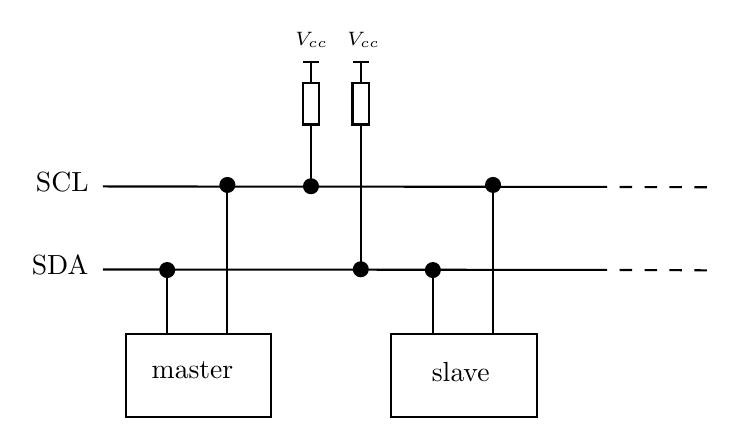
\begin{tikzpicture}[x=0.75pt,y=0.75pt,yscale=-1,xscale=1]
%uncomment if require: \path (0,300); %set diagram left start at 0, and has height of 300

%Straight Lines [id:da01486144209028284] 
\draw    (120,110) -- (357,110.2) ;
%Straight Lines [id:da9192669005866818] 
\draw  [dash pattern={on 4.5pt off 4.5pt}]  (357,110.2) -- (411,110.4) ;
%Straight Lines [id:da7272924823771425] 
\draw    (120,150) -- (357,150.2) ;
%Straight Lines [id:da6740141101838166] 
\draw  [dash pattern={on 4.5pt off 4.5pt}]  (357,150.2) -- (411,150.4) ;
%Shape: Rectangle [id:dp3448537161491223] 
\draw   (131,181) -- (201,181) -- (201,221) -- (131,221) -- cycle ;
%Shape: Rectangle [id:dp550508035925791] 
\draw   (259,181) -- (329,181) -- (329,221) -- (259,221) -- cycle ;
%Straight Lines [id:da6558849320962756] 
\draw    (151,150.27) -- (151,181) ;
\draw [shift={(151,150.27)}, rotate = 90] [color={rgb, 255:red, 0; green, 0; blue, 0 }  ][fill={rgb, 255:red, 0; green, 0; blue, 0 }  ][line width=0.75]      (0, 0) circle [x radius= 3.35, y radius= 3.35]   ;
%Straight Lines [id:da5049320053635051] 
\draw    (180,109.27) -- (180,181) ;
\draw [shift={(180,109.27)}, rotate = 90] [color={rgb, 255:red, 0; green, 0; blue, 0 }  ][fill={rgb, 255:red, 0; green, 0; blue, 0 }  ][line width=0.75]      (0, 0) circle [x radius= 3.35, y radius= 3.35]   ;
%Straight Lines [id:da8872527611539733] 
\draw    (279,150.27) -- (279,181) ;
\draw [shift={(279,150.27)}, rotate = 90] [color={rgb, 255:red, 0; green, 0; blue, 0 }  ][fill={rgb, 255:red, 0; green, 0; blue, 0 }  ][line width=0.75]      (0, 0) circle [x radius= 3.35, y radius= 3.35]   ;
%Straight Lines [id:da5785404530635856] 
\draw    (308,109.27) -- (308,181) ;
\draw [shift={(308,109.27)}, rotate = 90] [color={rgb, 255:red, 0; green, 0; blue, 0 }  ][fill={rgb, 255:red, 0; green, 0; blue, 0 }  ][line width=0.75]      (0, 0) circle [x radius= 3.35, y radius= 3.35]   ;
%Shape: Rectangle [id:dp1582668927496278] 
\draw   (216.28,60) -- (224.28,60) -- (224.28,80.16) -- (216.28,80.16) -- cycle ;
%Shape: Rectangle [id:dp5921011931609002] 
\draw   (240.28,60) -- (248.28,60) -- (248.28,80.16) -- (240.28,80.16) -- cycle ;
%Straight Lines [id:da11835655819703916] 
\draw    (216.28,50) -- (224.28,50) ;
%Straight Lines [id:da24500119650448204] 
\draw    (240.28,50) -- (248.28,50) ;
%Straight Lines [id:da4759484666860192] 
\draw    (220.28,80.16) -- (220.28,109.89) ;
\draw [shift={(220.28,109.89)}, rotate = 90] [color={rgb, 255:red, 0; green, 0; blue, 0 }  ][fill={rgb, 255:red, 0; green, 0; blue, 0 }  ][line width=0.75]      (0, 0) circle [x radius= 3.35, y radius= 3.35]   ;
%Straight Lines [id:da1351568499276985] 
\draw    (244.28,80.16) -- (244.28,149.89) ;
\draw [shift={(244.28,149.89)}, rotate = 90] [color={rgb, 255:red, 0; green, 0; blue, 0 }  ][fill={rgb, 255:red, 0; green, 0; blue, 0 }  ][line width=0.75]      (0, 0) circle [x radius= 3.35, y radius= 3.35]   ;
%Straight Lines [id:da32454229225190967] 
\draw    (244.28,50.43) -- (244.28,60.16) ;
%Straight Lines [id:da2779443621627411] 
\draw    (220.28,50.08) -- (220.28,59.81) ;

% Text Node
\draw (142,193) node [anchor=north west][inner sep=0.75pt]   [align=left] {master};
% Text Node
\draw (277,193) node [anchor=north west][inner sep=0.75pt]   [align=left] {slave};
% Text Node
\draw (86.28,102) node [anchor=north west][inner sep=0.75pt]   [align=left] {SCL};
% Text Node
\draw (84.28,142) node [anchor=north west][inner sep=0.75pt]   [align=left] {SDA};
% Text Node
\draw (211.28,34) node [anchor=north west][inner sep=0.75pt]  [font=\scriptsize] [align=left] {$\displaystyle V_{cc}$};
% Text Node
\draw (236.28,34) node [anchor=north west][inner sep=0.75pt]  [font=\scriptsize] [align=left] {$\displaystyle V_{cc}$};


\end{tikzpicture}}
    \caption{Oppkobling av en I2C-buss}
    \label{fig:app-I2cbuss}
\end{figure}
\subsection*{Start condition}

\verb|SCL| og \verb|SDA| er høye når bussen ikke er i bruk. En overføring startes ved at en master genererer en start condition på busslinjene. Start conditionet består av at masteren trekker \verb|SDA| lav, etterfulgt av \verb|SCL|. Når begge disse linjene er lave, vil masteren sette første databit på \verb|SDA|, før \verb|SCL| går høy for å signalisere til slavene på bussen at \verb|SDA| kan leses. Etter dette er overføringen i gang. En start condition er illustrert i figur \ref{fig:app-startcond-I2C}.

\begin{figure}
    \centering
    

\tikzset{every picture/.style={line width=0.75pt}} %set default line width to 0.75pt        

\resizebox{.65\textwidth}{!}{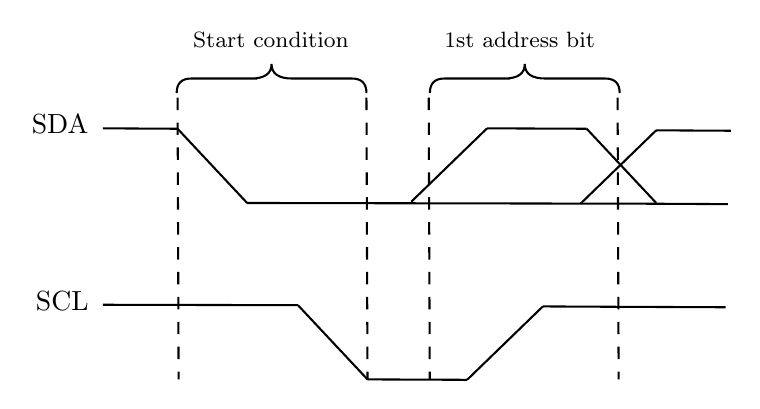
\begin{tikzpicture}[x=0.75pt,y=0.75pt,yscale=-1,xscale=1]
%uncomment if require: \path (0,300); %set diagram left start at 0, and has height of 300

%Straight Lines [id:da754152478497383] 
\draw    (120,178) -- (214,178.2) ;
%Straight Lines [id:da5755051872991086] 
\draw    (120,93) -- (156,93.2) ;
%Straight Lines [id:da18621949860045262] 
\draw    (189.5,128.96) -- (385.11,129.32) ;
%Straight Lines [id:da30636622752695053] 
\draw  [dash pattern={on 4.5pt off 4.5pt}]  (156,78.2) -- (156.5,213.96) ;
%Straight Lines [id:da029169460430886973] 
\draw  [dash pattern={on 4.5pt off 4.5pt}]  (247,78.2) -- (247.5,213.96) ;
%Straight Lines [id:da5522159141323546] 
\draw    (156,93.2) -- (189.5,128.96) ;
%Straight Lines [id:da37511562129003284] 
\draw    (332,178.8) -- (372,179) ;
%Straight Lines [id:da8788359359228113] 
\draw    (386.61,93.96) -- (422.61,94.16) ;
%Straight Lines [id:da3364691146922649] 
\draw    (268.61,128.36) -- (305.11,93) ;
%Straight Lines [id:da37121966753151514] 
\draw    (214,178.2) -- (247.5,213.96) ;
%Straight Lines [id:da9414953012609943] 
\draw    (295.5,214.16) -- (332,178.8) ;
%Straight Lines [id:da03660056007986512] 
\draw    (350.11,129.32) -- (386.61,93.96) ;
%Straight Lines [id:da45241154209117673] 
\draw    (353.11,93.2) -- (386.61,128.96) ;
%Straight Lines [id:da30120485744606595] 
\draw  [dash pattern={on 4.5pt off 4.5pt}]  (277,78.2) -- (277.5,213.96) ;
%Straight Lines [id:da3221706678341618] 
\draw  [dash pattern={on 4.5pt off 4.5pt}]  (368,78.2) -- (368.5,213.96) ;
%Straight Lines [id:da09132268721503434] 
\draw    (247.5,213.96) -- (295.5,214.16) ;
%Straight Lines [id:da48107873389756217] 
\draw    (305.11,93) -- (353.11,93.2) ;
%Straight Lines [id:da10377095903464073] 
\draw    (372,179) -- (420,179.2) ;
%Straight Lines [id:da21177934974706814] 
\draw    (385.11,129.32) -- (421.11,129.52) ;
%Shape: Brace [id:dp27010777384965223] 
\draw   (247,76) .. controls (247,71.33) and (244.67,69) .. (240,69) -- (211.28,69) .. controls (204.61,69) and (201.28,66.67) .. (201.28,62) .. controls (201.28,66.67) and (197.95,69) .. (191.28,69)(194.28,69) -- (162.56,69) .. controls (157.89,69) and (155.56,71.33) .. (155.56,76) ;
%Shape: Brace [id:dp14282895734173207] 
\draw   (369,76) .. controls (369,71.33) and (366.67,69) .. (362,69) -- (333.28,69) .. controls (326.61,69) and (323.28,66.67) .. (323.28,62) .. controls (323.28,66.67) and (319.95,69) .. (313.28,69)(316.28,69) -- (284.56,69) .. controls (279.89,69) and (277.56,71.33) .. (277.56,76) ;

% Text Node
\draw (86.28,170) node [anchor=north west][inner sep=0.75pt]   [align=left] {SCL};
% Text Node
\draw (84.28,85) node [anchor=north west][inner sep=0.75pt]   [align=left] {SDA};
% Text Node
\draw (162,45) node [anchor=north west][inner sep=0.75pt]  [font=\footnotesize] [align=left] {Start condition};
% Text Node
\draw (283,45) node [anchor=north west][inner sep=0.75pt]  [font=\footnotesize] [align=left] {1st address bit};


\end{tikzpicture}}
    \caption{ Start condition, og første adressebit, på I2C-buss.}
    \label{fig:app-startcond-I2C}
\end{figure}

\subsection*{Overføring}

For at hvert bit skal overføres korrekt, må det være riktig bit på \verb|SDA| i det \verb|SCL| går fra lav til høy. Hver slave taster \verb|SDA|-linjen for hver stigende anke på \verb|SCL|-linjen. Begge linjene styres i utgangspunktet av masteren, men hvis en slave ikke er i stand til å motta flere bit, kan den tvinge masteren til å avvente videre sending ved å trekke \verb|SCL| lav (denne type oppførsel kalles \textit{clock stretching}). 

Hver byte overført over I2C må bekreftes av en mottaker. Man sier gjerne at mottakeren sender en \verb|ACK| (Acknowledgement) tilbake. Dette gjøres ved at masteren slipper \verb|SDA|-linjen etter det åttende bit-et den har sendt. Deretter vil masteren generere en ekstra klokkepuls på \verb|SCL|; og nå er det opp til mottakeren å trekke \verb|SDA| lav for å signalisere at den har mottatt bytet. Hvis masteren ikke merker at \verb|SDA| trekkes lav, vil den avbryte sendingen.


\subsection*{Adressering}


For å signalisere hvilken enhet masteren ønsker å snakke med, vil hver enhet ha en unik adresse på bussen. For sensorer (slik som akselerometeret og magnetometeret på micro:bit-en) vil adressen stort sett være forhåndsbestemt fra fabrikanten uten mulighet til å endres.

Etter at en start condition har blitt generert, vil det første bytet masteren sender bestå av 2 adressebit, og ett retningsbit. Retningsbitet forteller om masteren ønsker å skrive til-, eller lese fra en mottaker. Retningsbitet vil være \verb|1| for en leseoperasjon, og \verb|0| for en skriveoperasjon. Så fremt 10-bits adressering ikke brukes, vil alle byte som følger etter dette første bytet, være data.

\subsection*{Arbitrering}

Dersom det finnes flere mastere på en buss, kan det hende at to mastere griper etter I2C-linjene samtidig. For å bli enige om hvem som får lov til å sende først, brukes mottakeradressen som meglingsmiddel.

I2C er en CSMA/CD+AMP protokoll (\textbf{Ca}rrier \textbf{S}ense \textbf{M}ultiple \textbf{A}ccess
with \textbf{C}ollision \textbf{D}etection and \textbf{A}rbitration by \textbf{M}essage \textbf{P}riority). Dette betyr at hver I2C-master vil sample busstiltanden og sammenligne med det den selv ønsket å putte på linjene. Hvis to mastere begynte en overføring samtidig, og en av dem ønsket å sende et høyt bit, mens den andre ønsket å sende et lavt bit - vil masteren som sender det lave bitet trekke \verb|SDA| lav. Dette vil masteren som ønsket å sende et høyt bit merke, og dermed avslutte sendingen. Fordi adressebytet sendes først, vil den masteren som addresserer den laveste adressen vinne (så lenge de ikke referer til samme adresse).


\subsection*{Trivia}
Andre protokoller som for eksempel CAN (\textbf{C}ontroller \textbf{A}rea \textbf{N}etwork) støtter også forskjellige meldingsprioriteter, noe som er implementert ved at den meldingen som har lavest ID alltid får sende først. Denne type protokoll har navnet CSMA/CD+AMP (\textbf{Ca}rrier \textbf{S}ense \textbf{M}ultiple \textbf{A}ccess
with \textbf{C}ollision \textbf{D}etection and \textbf{A}rbitration by \textbf{M}essage \textbf{P}riority)

\cprotect\section{Appendiks - Debugging med OpenOCD}\label{app:Debugging}

For å debugge micro:bit-en kan vi bruke et program som heter \href{https://openocd.org/}{OpenOCD} (Open On-Chip Debugger). Dette programmet kommuniserer med interface MCUen, og gjør det mulig å hente ut nyttig informasjon direkte fra target MCU. Programmet skal allerede være installert på lab-PCene, men kan installeres med:

\verb|sudo apt install openocd|

\subsection*{OpenOCD med GDB}

For å starte programmet skriv inn kommandoen:

\verb|openocd -f interface/cmsis-dap.cfg -f target/nrf52.cfg|

Denne kommandoen forteller OpenOCD at vi ønsker å snakke til en nRF52-chip, som er target MCUen vår. (\verb|interface/cmsis-dap.cfg| forteller bare at vi ønsker å bruke programvaren som kjører på interface MCUen, og er ikke viktig for oss.) OpenOCD vil så koble til micro:bit-en og starte en GDB-server som vi ønsker å koble oss til. 

Åpne så et nytt terminalvindu og naviger deg til oppgavemappen du ønsker å debugge. Bygg så programmet med \verb|make debug|. Dette er viktig for at GDB skal kunne lese programmet vårt. Skriv deretter inn kommandoen:

\verb|/opt/arm-none-eabi-12.2/bin/arm-none-eabi-gdb .build_system/main.elf|

Dette vil starte GDB og laste inn programmet du nettopp har bygget. Du kan erstatte \verb|main.elf| med programmet du ønsker å debugge. Det siste steget er å koble seg til GDB-serveren OpenOCD har startet for oss. Dette kan vi gjøre med å skrive den følgende kommandoen i GDB:

\verb|target extended-remote localhost:3333|

Du vil nå være koble til GDB-serveren, og vil kunne debugge micro:bit-en som om koden kjørte på din egen maskin. (Se Øving om GDB)

\subsection*{OpenOCD med VSCode}

Mange foretrekker å debugge og programmere i en moderne IDE som VSCode. Vi har derfor laget et utviklingsmiljø som dere kan laste ned. Utviklingsmiljøet baserer seg på OpenOCD og utvidelsen \href{https://open-vsx.org/extension/marus25/cortex-debug}{Cortex-Debug}. For å bruke dette utviklingsmiljøet må du laste ned vscode-utviklingsmiljøet fra Blackboard og pakke ut filene i oppgavenmappen du ønsker å debugge. Sørg for at \verb|.vscode|-mappen ligger i samme mappe som \verb|.build_system|. Begge disse mappene er "skjulte", som vil si at du må bruke \verb|ls -a| for å se dem i et terminalvindu. Åpne så oppgavemappen i VSCode (dette kan du gjøre med kommandoen \verb|code .| ). VSCode vil så be deg om å laste ned utvidelsen \verb|Cortex-debug|. Etter å ha installert denne kan du trykke på \verb|Run and Debug|-fanen for å så debugge programmet. Se VSCode sin dokumentasjon via \href{https://code.visualstudio.com/Docs/editor/debugging}{denne lenken her} for bruk av debug-verktøyet.

% \cprotect\section{Appendiks - Kort om BLE}\label{app:ble}

% BLE (\textbf{B}luetooth \textbf{L}ow \textbf{E}nergy), eller Bluetooth 4.2 er en versjon av Bluetooth som er skreddersydd for applikasjoner som skal trekke lite strøm. Første versjon av BLE (Bluetooth 4.0) ble gitt ut i 2010, og siden da har BLE blitt spesielt populært i mange forskjellige industrier. Hovedpådragdriveren bak dette finner man i utviklingen av smarttelefoner (spesielt Samsung og Apple). BLE er spesielt attraktivt, fordi standarden lar en tilpasse protokollen til sine egne formål, i motsetning til Bluetooth Classic, som kun definerte et snevert sett av use cases.

% Ulempen med BLE, er at den i forhold til Bluetooth Classics, har en mye mindre overføringsrate. Applikasjoner som det å høre på musikk over BLE er nærmest umulig å få til over en BLE-kobling. Til tross for at moduleringsraten til en BLE-radioenhet ligger på rundt 1 Mbps, introduserer protokollen i seg selv en betydelig mengde overhead som begrenser mulig senderate. I vårt tilfelle kan en nRF51822 sende opp til 6 datapakker hvert connection interval (tiden for en dataoverføring mellom to enheter). Hver datapakke kan inneholde opp til 20 brukerdefinerte byte. Den raskeste man kan sette et connection interval til å være er 7.5 \si{\milli\s}. Dette gir en teoretisk maksgrene på:

% \begin{align*} \frac{6 \cdot 20 \cdot 8 \text{bit}}{7.5 \si{\milli\s}} = 128 \ \si{\kilo}\text{bit/}\si{\s} \end{align*}

% I tillegg til dette, vil BLE alltid prøve å sende tapte pakker på nytt, kollisjoner kan skje på båndet, radioenheten kan være opptatt ogsv. Dette betyr i praksis at man kan forvente omlag 40-80 kbps. Dette relativt lavt for vanlig dataoverføring, men så er det heller ikke det BLE er laget for å gjøre - når det kommer til lavt strømtrekk er dette veien å gå.

% Fra et teknisk synspunkt har Bluetooth-stakken endret seg mye fra Bluetooth Classic til BLE; så mye at det er egentlig er snakk om to forskjellige protokoller som begge har "Bluetooth" i navnet. De har veldig forskjellig fokusområder, og er heller ikke i stand til å snakke direkte med hverandre. Det er ikke viktig i dette faget, men for de spesielt interreserrte, er forskjellene i Bluetooth-stakkene illustrert i figur .... "BR/EDR" står for \textbf{B}asic \textbf{R}ate \textbf{E}nchanced \textbf{D}ata \textbf{R}ate, og er betegnelsen vi bruker for Bluetooth classic.

% Mens Bluetooth classic deler 2.4 GHz ISM-båndet inn i 79 kanaler, nøyer BLE seg med å dele det samme båndet inn i 40 kanaler (se figur ....) Kanalene 37, 38 og 39 er reservert for kringkasting over GAP, mens GATT står fritt til å hoppe mellom de andre kanalene.

% Når det kommer til nettverkstoplogier er BLE ganske liberal i hva den tillater. Det er mulig å kringkaste til alle som vil høre på, over en eller flere av kringkastingskanalene. Dette tillater en enhet å sende informasjon til flere mottakere samtidig. Dette begrenser derimot en enhet til å kun sende; for toveis kommunikasjon må man etablere en kobling.

% Alle koblinger i BLE involverer en central, og en peripheral. Det er ikke mulig å sende til flere mottakere samtidig når man bruker en tilkobling. For å komme rundt dette, har man siden Bluetooth 4.1 kunnet konfiguere en fysisk enhet til å anta enhver kombinasjon av central og peripheral man ønsker. Det er dermed mulig å ha en enhet som fungerer både som en central og peripheral på en gang. Hver av disse rolleinstansene står da fritt til å gjøre koblinger med andre enheter rundt seg.


% Et sentral konsept i Bluetooth Low Energy er GATT (\textbf{G}eneric \textbf{A}ttribute \textbf{P}rofile). Denne delen av standarden definerer en klient- server- arkitektur, som arrangerer attributter i forskjellige karakteristikker som til sammen implementerer en eller flere tjenester. Det meste av informasjonsoverføring av betyding foregår over GATT, og er en av de viktigste grunnene til at BLE er en såpass allsi


